%%% Local Variables:
%%% mode: latex
%%% TeX-master: t
%%% End:

\documentclass{article}

\usepackage{fullpage}
\usepackage[utf8]{inputenc}
\usepackage{listings}
\usepackage{caption}
\usepackage{subcaption}
\usepackage[svgnames]{xcolor}
\usepackage{amssymb}
\usepackage{amsmath}
\usepackage{fancyhdr}
\usepackage{lastpage}
\usepackage{parskip}
\usepackage{abstract}
\usepackage{gensymb}
\usepackage{url}
\usepackage{float}
\usepackage{enumitem}
\usepackage{amstext}
\usepackage{fancybox}
\usepackage{amsmath}
\usepackage{graphicx}
%\usepackage{subfigure}
\usepackage[bottom]{footmisc}
\usepackage{hyperref}
\usepackage{tikz}
\usepackage{makecell}
\usepackage{tabulary}
\usepackage{pdfpages}
\usepackage{verbatim}
\usepackage{tikz}
\usetikzlibrary{positioning}
\usetikzlibrary{arrows}
\pagenumbering{gobble}

\setcounter{secnumdepth}{3} % only chapter and sections will be numbered
\setcounter{tocdepth}{3}    % entries down to \subsubsections in the TOC

\definecolor{Brown}{cmyk}{0,0.81,1,0.60}
\definecolor{OliveGreen}{cmyk}{0.64,0,0.95,0.40}
\definecolor{CadetBlue}{cmyk}{0.62,0.57,0.23,0}
\definecolor{lightlightgray}{gray}{0.95}
\definecolor{lightgray}{gray}{0.85}
\definecolor{sh_comment}{rgb}{0.12, 0.38, 0.18}
\definecolor{sh_keyword}{rgb}{0.37, 0.38, 0.75}
\definecolor{sh_string}{rgb}{0.06, 0.10, 0.98}

\lstset{
basicstyle=\small\ttfamily,
stringstyle=\color{sh_string},
keywordstyle = \color{sh_keyword}\bfseries,
commentstyle=\color{sh_comment},
backgroundcolor=\color{lightlightgray},
frame=single,
rulecolor=\color{lightgray},
framesep=3pt,
numbersep=5pt,
xleftmargin=10pt,
xrightmargin=10pt,
showspaces=false,
showstringspaces=false,
tabsize=4,
aboveskip=5pt,
belowskip=5pt,
lineskip=2pt,
captionpos=b,
numbers=left,
numberstyle=\tiny,
stepnumber=1,
numbersep=100pt,
breaklines,
numbersep=5pt,
breakatwhitespace=false,
showspaces=false,
showtabs=false
}

\lstnewenvironment{cpp}[0]{
\lstset{language=C++,
}}
{}


\lstnewenvironment{assembly}[0]{
\lstset{language={[x86masm]Assembler},
}}
{}


\title{Operating System Notes}
\author{December 2014}
\date{}

\begin{document}

\maketitle
\tableofcontents
\pagebreak

\section{Compiler optimization}
\emph{1. You can list and describe three source code transformations the compiler can perform to achieve higher performance.}

\begin{enumerate}
	\item Loop-optimization: Move loop-invariant variables outside the loop.
	\item Dead code removal.
	\item Subexpression elimination: $(x + y) / 3.0 - (x + y)\rightarrow temp = y+x;\;\; temp/3.0-temp$
	\item Replacing instructions with more efficient ones. For instance, x = x * 2 is likely faster performed by bitshifting
\end{enumerate}

Primarily optimizing either for (run) time or for space.


\section{Programming methodologies}
\emph{2. You can apply standard programming methodologies and tools such as test-driven development, build systems, debuggers.}

\begin{description}
\item[Test-driven development (TDD)] \ \\
Software development process. Cycle:
\begin{enumerate}
\item Write initially failing test defined desired functionality
\item Implement functionality, passing test
\end{enumerate}

\item[Build systems] \ \\
Automating common tasks as:
\begin{itemize}
\item Compiling computer source code into binary code
\item Packaging binary code
\item Running automated tests
\item Deploying to production systems
\item Creating documentation and/or release notes
\end{itemize}

\item[Debuggers] Process of finding and reducing number of bugs in program or part of hardware.
\end{description}


\section{Compilation toolchain}
\emph{3. You can explain the role of each component of a compilation toolchain used in system programming and how the components interact.}

\begin{enumerate}
	\item Source file(s) are handled by the preprocessor, which turn them into \textbf{translation units}:
	\begin{itemize}
		\item The preprocesser recursively includes files marked by \#include
		\item The preprocesser expands macros such as \#if, \#define, \#ifdef
	\end{itemize}
	Translation units consists of declarations and definitions.
	\item Each translation unit is then \emph{compiled} into object files
	\item Object files can then, together with (static) libraries, be linked into executables.
\end{enumerate}

\textbf{Remember} that there are both \emph{static} and \emph{dynamic} libraries. Static are linked into the executable, whereas dynamic can be changed (updated) with time (dynamic linked).


\section{Memory leaks}
\emph{4. You can explain in your own words how memory leaks can occur in systems with dynamic memory management and give examples of two approaches to prevent them.}

\subsection{How they can occur}
\begin{itemize}
	\item In the C standard library, one can call \texttt{malloc()} to get a pointer to the memory of the requested size.
 If one deletes the pointers to the allocated data, without freeing the memory block before, this is a memory leak.

 	\item Memory fragmentation
\end{itemize}


\subsection{Strategies to prevent them}
\begin{itemize}
	\item Garbage collection. Detect data objects that cannot be used by the program in the future, and free the resources occupied by these.
	\item Always add free after a malloc and then put code that uses the variable in between.
	\begin{cpp}
int *p = (int*) malloc ( sizeof(int) * n );
//Put code here..
free (p);
	\end{cpp}
	\item Never use allocated pointer for doing stuff. Instead use a copy and use that in code. Copy the pointer...
	\begin{cpp}
int *p_allocated = (int*) malloc ( sizeof(int) * n );
int *p_copy = p_allocated;
// do your stuff with p_copy, not with p_allocated!
// e.g.:
while (n--) { *p_copy++ = n; }
...
free (p_allocated);
	\end{cpp}
\end{itemize}


\section{Memory mapped I/O vs. I/O-instructions}
\emph{5. You can explain the difference between communicating with an I/O device using memory mapped I/O or I/O instructions.}
%%% Local Variables:
%%% mode: latex
%%% TeX-master: "../cheat-sheet"
%%% End:

% \emph{5. You can explain the difference between communicating with an I/O device using memory mapped I/O or I/O instructions.}

\textbf{Memory mapped I/O}: A device's memory is mapped to the CPU's memory address space, ie. the device's memory is manipulated in exactly the same way as regular memory.

\textbf{I/O instructions}: Processes can use I/O instructions, such as the \texttt{IN} and \texttt{OUT} instructions in the \texttt{x86} instruction set. Those two transfer data between I/O devices and registers/memory through the I/O ports of the CPU.



\section{CPU Terminology}
\emph{6. You can explain in your own words the following terms: processor, register, program counter, cache, I/O device, instruction set architecture.}

\begin{figure}[H]
  \centering
  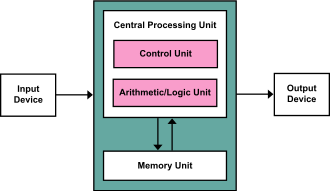
\includegraphics[width=8.0cm]{images/330px-Von_Neumann_Architecture.png}
  \caption{Von Neumann Architecture}
\end{figure}


\subsection{Processor}
There are different kinds of processors, the most widely used are
\begin{itemize}
	\item General purpose central processing units (CPUs, used in PCs)
	\item ASIC (application-specific integrated circuit)
	\item GPU (graphics processing units)
\end{itemize}

Operates in \textbf{cycles}:
\begin{itemize}
	\item Fetch instruction (using the PC/IP)
	\item Decode instruction (there are different \emph{addressing modes})
	\item Execute - Control Unit and ALU (Arithmetic/Logic Unit)
\end{itemize}
(This is the so-called three-stage pipeline. There is also the modern superscalar CPU (see page 21 in DJ Tanenbaum's book))

\textbf{Word size} - Modern PCs use a word-size of 64 bits. Embedded systems using microcontrollers often have a smaller word size (modern ones have down to 8 bit)

\subsection{Register}
Lulz

\subsection{Program counter / instruction pointer (PC/IP)}
So... yeah.

\subsection{Cache}
TODO: cache coherence - when there are multiple caches for multiple processors. These must be kept consistent.

\subsection{I/O device}

\subsection{Instruction set architecture (ISA)}
Well-defined software/hardware interface.

\begin{itemize}
	\item Functional definition - Operations and storage locations supported by hardware. With Intel's Ivy Bridge chip-architecture came the operation RdRand for instance, which is an operation that returns a hardware-generated random number.
	\item Documentation of how to use the instructions (see ABI below?).
\end{itemize}

(TODO: application binary interface (ABI). I believe this is contained within ISA. This defines the calling conventions for the architecture - for instance how system calls are carried out)


\section{Basic processor functionality}
\emph{7. You can explain the basic workings of a processor and outline the steps involved in executing an instruction.}
TODO


\section{Interrupts}
\emph{8. You can explain in your own words how interrupts are handled in the processor.}

When the processor gets interrupted, it
\begin{enumerate}
	\item Halts execution of the current thread
	\item Stores the current state (TODO: the book says that this ranges from storing only the IP-register, to storing \emph{all} registers of the thread).
	\item Executes interrupt handler
	\item Resumes thread execution
\end{enumerate}

Two types of interrupts:
\begin{itemize}
	\item \textbf{Hardware} - when a disk-read, keyboard input, clock (timing), scanned document is ready. Sent via the Bus.
	An Interrupt Controller handles this and issues interrupt for CPU.
	(if there are several HW-interrupts sent simultaneously, the ones with lower priorities keep sending the signal)

	\item \textbf{Software} - Either when an `interrupt instruction' is executed, or when an exception is thrown. (exceptions can be from other processors as well!)

\end{itemize}

The halting of execution and storing of state is much more complex on modern, superscalar CPUs (see page 21 in DJ Tanenbaum's)


\section{Indirect addressing (assembly)}
\emph{9. You can show with assembly code how the stack pointer, or a general purpose register, can be used to perform indirect addressing of data structures.}
%%% Local Variables:
%%% mode: latex
%%% TeX-master: "../cheat-sheet"
%%% End:

% 9. You can show with assembly code how the stack pointer, or a general purpose register, can be used to perform indirect addressing of data structures.

Consider
\begin{lstlisting}[language=C]
struct person {
  double height;
  int    age;
}

struct person turing = (struct person*)malloc(sizeof(struct person));
turing->age = 40;
turing->name = "Alan Turing";
\end{lstlisting}

We can now use indirect addressing to access the fields of the struct:

\begin{lstlisting}[language={[x86masm]Assembler}]
; eax now holds the address of `turing'
mov turing, %eax

; mov 1.0 to the first field of the struct (the double literal is not valid assembly)
mov $1.0, (%eax)

; mov 2 to the second field which is offset by 8 bytes (size of the double)
mov $2, 8(%eax)
\end{lstlisting}


Generally:
\begin{description}
\item[Indirect addressing:] \texttt{(\%eax)}
\item[Base pointer addressing:] \texttt{4(\%eax)}
\end{description}

The general form of memory address references is this:

\texttt{ADDRESS\_OR\_OFFSET(\%BASE\_OR\_OFFSET,\%INDEX,MULTIPLIER)}

\texttt{FINAL ADDRESS = ADDRESS\_OR\_OFFSET + \%BASE\_OR\_OFFSET + MULTIPLIER * \%INDEX}

See Bartlett chapter 3



\section{Memory hierarchy}
\emph{10. You can draw a figure showing how the memory hierarchy of a modern computer with the processor(s), cache levels, memory and storage}

\begin{center}
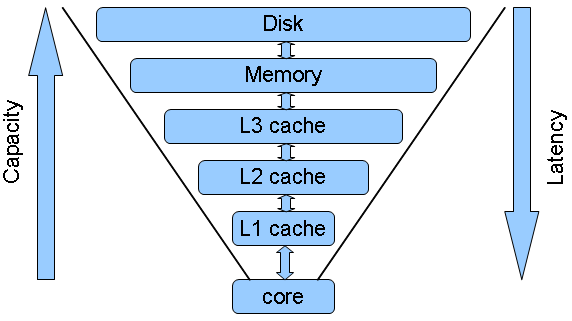
\includegraphics[width=5.0cm]{images/cpu_cache_structure.png}
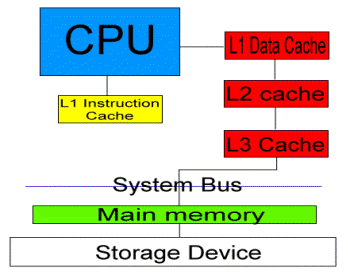
\includegraphics[width=5.0cm]{images/CPU-Cache-System.png}

Simplified overviews of CPU, registers, caches and memory
\end{center}

\emph{L1} is often local for each CPU, whereas \emph{L2} and/or \emph{L3} are/is often shared between multiple CPUs.

\emph{Extremely} important: When you draw the storage, remember to draw it as a cylinder\footnote{due to historical reasons}!


\section{Interrupt handler}
\emph{11. You can write pseudocode showing how to implement an interrupt handler.}
TODO


\section{Cache performance}
\emph{12. You can demonstrate with pseudo code how the memory access pattern of a program can greatly influence cache performance.}
%%% Local Variables:
%%% mode: latex
%%% TeX-master: "../cheat-sheet"
%%% End:

By avoiding cache misses (thus increasing cache hits) we can speed up memory lookups. When the CPU fetches memory it will fetch nearby elements into the cache as well because they are typically used together. If we fetch memory from scattered places its unfriendly for the cache.

For instance, iterating a two-dimensional array:

\begin{lstlisting}
nums = [[1, 2],
        [3, 4]]
// consider that `nums' this stored in memory as [1, 2, 3, 4]
\end{lstlisting}

If we iterate column-wise, and the cache fetches a single element ahead we get something like

\begin{lstlisting}
for col = 0 to 1:
    for row = 0 to 1:
        print nums[row][col]
\end{lstlisting}

This will result in accesses in this order: \texttt{nums[0][0] (1), nums[1][0] (3), nums[0][1] (2), nums[1][1] (4)}. If the CPU fetches and caches one address ahead then the first memory access fetches \texttt{nums[0][0] (1)} and caches \texttt{nums[0][1] (2)} but the next fetch is actually \texttt{nums[0][0] (3)} which results in a cache miss.

We can get two cache hits and two memory lookups instead of four memory lookups if we iterate row-wise instead!



\section{Privilege levels}
\emph{13. You can explain the concept of privilege levels and show three examples of operations which should be permitted only at the most privileged level.}
% 13. You can explain the concept of privilege levels and show three examples of operations which should be permitted only at the most privileged level.
Processes run under privilege level from 0 (most privileged) through 3 (least privileged). The assigned level controls what resources the process has access to, such as memory, IO, special instructions. Kernel code runs in ring 0 and general user programs run in level 3, all levels are not always used (for instance 1 and 2 are unused in Linux). Level 0 is essentially kernel mode. Current privilege level is stored in the \texttt{CPL} register.

Operations only permitted in level 0 (many of these are just system calls)
\begin{itemize}
\item Process creation
\item Process termination
\item Disable interrupts
\item Modify memory map (virtual memory)
\item File writing
\item File reading
\end{itemize}

%%% Local Variables:
%%% mode: latex
%%% TeX-master: "cheat-sheet"
%%% End:



\section{Message passing}
\emph{14. You can explain in your own words and in text and with your own commented examples, how message passing can be used to coordinate processes.}
TODO


\section{Kernel types}
\emph{15. You can explain in your own words the differences between a monolithic operat-
ing system, a micro-kernel operating system, and an exo-kernel based operating
system.}

\subsection{Monolithic}
\begin{itemize}
\item Entire operating system is working in kernel mode.
\item Defines a high-level virtual interface over computer hardware.
\item A set of primitives or system calls implement all operating system services such as process management, concurrency, and memory management.
\item Device drivers can be added to the kernel as modules.
\end{itemize}

\subsection{Microkernel}
\begin{itemize}
\item Near-minimum amount of software that can provide the mechanisms needed to implement an OS.
\item Mechanisms include low-level address space management, thread management, and inter-process communication (IPC).
\item Microkernel is the only software executing in kernel mode.
\item Other functions, such as device drivers, protocol stacks and file systems, are removed from the microkernel to run in user mode.
\end{itemize}

\begin{figure}[H]
  \centering
  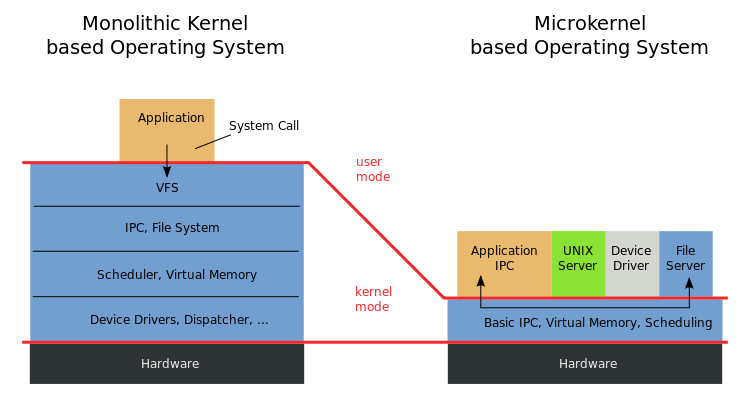
\includegraphics[scale=0.5]{images/mono-microkernel.png}
  \caption[Caption for LOF]{Overview of exo-kernel\footnotemark}
\end{figure}
\footnotetext{\url{https://en.wikipedia.org/wiki/Microkernel\#mediaviewer/File:OS-structure.svg}}

\subsection{Exokernel}
\begin{itemize}
\item Force as few abstractions as possible on developers, enabling them to make as many decisions as possible about hardware abstractions.

\item Tiny, since functionality is limited to ensuring protection and multiplexing of resources.

\item The kernel only ensures that the requested resource is free, and the application is allowed to access it.

\item Allows direct access to hardware from user space programs
\end{itemize}

\begin{figure}[H]
  \centering
  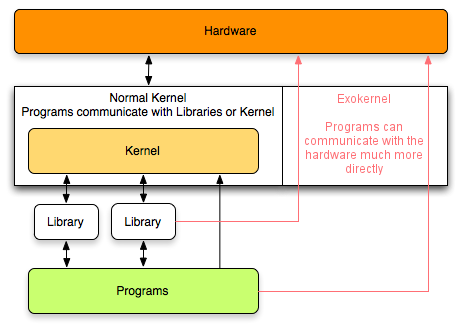
\includegraphics[scale=0.5]{images/exokernel.png}
  \caption[Caption for LOF]{Overview of exo-kernel\footnotemark}
\end{figure}
\footnotetext{\url{https://en.wikipedia.org/wiki/Exokernel\#mediaviewer/File:Exokernel\_revised(english).png}}


\section{Uni-processor system}
\emph{16. You can explain in your own words how multiple processes can share the same CPU.}
This is possible by context switching between the execution of the processes or threads (this is called \textbf{multitasking}). The context switch stores the current state of the process, so that the execution of it can be resumed at a later point in time.

This is most likely implemented with a preemptive scheduler on PCs, as programs would otherwise be able to hold on to the CPU. So the scheduler decides when to switch between processes.

\begin{center}
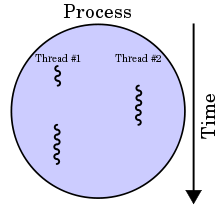
\includegraphics[width=5.0cm]{images/220px-Multithreaded_process.png}

A process with two threads - run on a single CPU
\end{center}

The above can also be performed between several processes, and thus a single CPU can execute several processes ``at the same time'' (at least it might appear so to the user).


\section{Multi-processor system}
\emph{17. You can explain in your own words how multiple processes can share a set of CPUs.}
With multiple CPUs one can, instead of switching out a running process to let another run, simply run the other process on another CPU.

Given the individual process address space and individual call stack for each thread, multiple processes are able to run in parallel on several CPUs without affecting the states of one another.


\section{Thread states}
\emph{18. Assume a thread can be in three different states: running, blocked, ready. You can draw a diagram of your own showing the transitions between states and explain in text and in your own words what each transition means.}
%%% Local Variables:
%%% mode: latex
%%% TeX-master: "cheat-sheet"
%%% End:

When a process blocks, it does so because logically it cannot continue, typically because it is waiting for input that is not yet available.

It is also possible for a process that is conceptually ready and able to run to be stopped because the operating system has decided to allocate the CPU to another process for a while.

These two conditions are \emph{completely different}. In the first case, the suspension is inherent in the problem (you cannot process the user' s command line until it has been typed). In the second case, it is a technicality of the system (not enough CPUs to give each process its own private processor).

The three possible states:
\begin{description}
\item[Running] Actually using the CPU at that instant
\item[Ready] Runnable; temporarily stopped to let another process run
\item[Blocked] Unable to run until some external event happens
\end{description}

\begin{figure}[H]
  \centering
  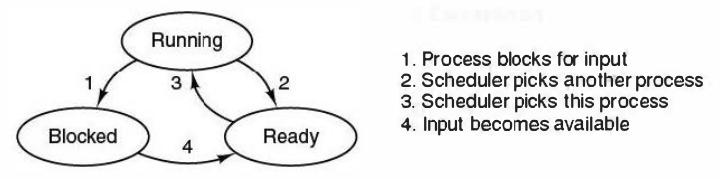
\includegraphics[scale=0.5]{images/thread_life}
  \caption{Transition diagram of thread states}
\end{figure}



\section{Operating system stack}
\emph{19. Given a schematic overview of the software stack of an operating system, you can label, in the diagram, key system parts. You can also explain in your own words and in text the purpose of those parts.}
TODO


\section{Key concepts}
\emph{20. Given reference literature, you can write down in text and in your own words definitions or explanations of the following concepts: Process; Address space; Interprocess communication; System call; Daemon; Thread; Critical section; Mutual exclusion; Semaphore; Mutex; Monitor; Condition variable; Message passing; Kernel mode; User mode; Pre-emtiveness; Race condition; Scheduling algorithm; System time; Device driver.}
\emph{24. Given reference literature, you can write down in text and in your own words definitions or explanations of the following concepts: Virtual machine; Virtual machine monitor; Atomic action; Swapping; Virtual memory; Paging; File system; File attribute.}
Given reference literature, you can write down in text and in your own words definitions or explanations of the following concepts:

\begin{description}
\item[Process Address space]
  The actual address space taken allocated to a process in a virtual address space.

\item[Interprocess communication]
  Can be done in numerous ways: files, message queues, semaphore, message passing, shared memory, pipes (IO), and more.

\item[System call]
  A program's request to the operating system to do an OS tasks

\item[Daemon]
  A process running in the background (``invisible''), can be a watchdog-like program, auto-updater, anti-virus, etc.

\item[Thread]
  Smallest ``unit'' known by the scheduler. Owned by a process. Threads of the same process share memory.

\item[Critical section]
  A piece of code that needs mutual exclusion. A critical \texttt{region} consists of multiple of these.

\item[Mutual exclusion]
  Ya kno dis

\item[Semaphore]
  P = request/take coconut, V = put coconut. Semaphore invariant: $\#P \le \#V + s$.

\item[Mutex]
  Binary semaphore, a simple lock/unlock mechanism

\item[Monitor]
  A construct (class, object, whatever) with mutual exclusion of methods

\item[Condition variable]
  A condition that a monitor can await to be signalled. In a Java monitor it's done via \texttt{wait} and \texttt{notify} and \texttt{notifyAll}. It's the mechanism by which a monitor can wait for a condition to be true without blocking the monitor.

\item[Message passing]
  Communication between objects in the same process or between different processes by use of so-called messages. Can be asynchronous or synchronous. Invoking a method on an object in Java is an example of message passing, and sending a signal from one process to another in unix with \texttt{kill} is another.

\item[Kernel mode]
  One of the two modes of operation of the CPU. In kernel mode all code executed is \textit{trusted} so it can access all memory, signal all processes, execute all instructions, etc.

\item[User mode]
  One of the two modes of operation of the CPU. In user mode code is not assumed to be \textit{trusted} so it is restricted to a certain memory space and possibly a limited subset of CPU instructions.

\item[Pre-emtiveness]
  A preemption happens when a process is suspended \textit{during} its execution, resulting in a \textit{context switch}, usually done by the scheduler. The intent is that the process will be resumed later.

\item[Race condition]
  Happens when two processes attempts to access/mutate a shared resources at the same time, such that unexpected behavior or corruption can occur.

\item[Scheduling algorithm]
  Algorithm that chooses which processes (or threads) to execute.

\item[System time]
  The computer's time ``counter''

\item[Device driver]
  Program that controls a hardware device and provides an interface to it (usually through the bus)

\item[Virtual machine]
  One machine providing multiple virtual machines (VM) to the next layer, such that multiple users can have their own, closed environment, while sharing the same resources.

\item[Virtual machine monitor]
  A hypervisor or virtual machine monitor (VMM) is a piece of computer software, firmware or hardware that creates and runs virtual machines.
\begin{figure}[H]
  \centering
  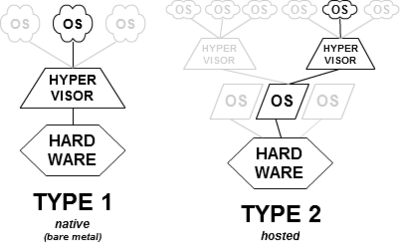
\includegraphics[scale=0.5]{images/hypervisor}
  \caption{Type-1 and type-2 hypervisors}
\end{figure}

\item[Atomic action]
  An instruction or set of instructions that cannot be interleaved by other processes, thus making it always completely done, or not started.

\item[Swapping]
  Memory management technique where a process is fully loaded into RAM to be run, and put back onto disk when idled.

\item[Virtual memory]
  Memory management technique in which a process is assigned \emph{virtual memory addresses} which are mapped by the operating system into physical memory locations, which could be either in RAM or on disk via paging. Allows programs to be run without being fully loaded into memory.

\item[Paging]
  Virtual memory is divided into fixed sized (512 bytes - 64KB) chunks called pages which are mapped to physical memory chunks (generally) of the same size. The MMU (memory management unit) translates addresses via a table.

\item[File system]
  A system by which the operating system distinguishes \emph{persistent} data stored on disk as separate units of coherent data, known as files.

\item[File attribute]
  Attributes attached to files such as being hidden, read-only, system critical, etc.

\end{description}


\section{Race conditions}
\emph{21. You can explain in your own words, in text and with your own examples how race conditions can occur in systems with multiple processors or systems with interrupts.}
TODO


\section{Mutual exclusion}
\emph{22. You can explain in your own words, in text and with your own commented examples, how busy wait methods can achieve mutual exclusion in systems with multiple CPUs.}
\emph{23. You can explain in your own words, in text and with your own commented examples, how blocking methods can achieve mutual exclusion in systems with multiple CPUs.}
% 22. You can explain in your own words, in text and with your own commented examples, how busy wait methods can achieve mutual exclusion in systems with multiple CPUs.
% 23. You can explain in your own words, in text and with your own commented examples, how blocking methods can achieve mutual exclusion in systems with multiple CPUs.

\subsection{Busy wait}
Uses the full resource of the thread to stay alive and continuously check for the critical section lock to become available.

Pseudo:
\begin{cpp}
int locked = 0;

void mutex_enter() {
  while (locked) { /* noop */ }
  locked = 1;
}

void mutex_exit() {
  locked = 0;
}
\end{cpp}

Usage
\begin{cpp}
mutex_enter();
/* critical section */
mutex_exit();
\end{cpp}

It is worth noting that one can also use the \texttt{TSL} (Test Set and Lock) or \texttt{CAS} (Compare And Swap) instructions to implement this.

\subsection{Blocking}
Puts the process to sleep and wakes it up from another process. Semaphores and monitors can do this. TODO: more?


%%% Local Variables:
%%% mode: latex
%%% TeX-master: "cheat-sheet"
%%% End:



\section*{Context switching}
Stores the state of the registers, as the rest will remain untouched by other processes (
TODO: mention individual 1) process address space and 2) call stack for each thread)


\section*{C - interrupts!}
TODO: fuck fuck fuck


\section*{C - storage classes (week 2)}
TODO: auto, extern, static and register!


\section*{Memory layout (week3)}
TODO: (memory areas) How are they laid out? In what order Where in memory?


\end{document}
